\begin{Q}
\textbf{Pretrained CLIP for Zero-Shot and Few-Shot Image Classification. 50 Points}

In this problem, you will use a \emph{pretrained} CLIP model for zero-shot and few-shot image classification, following the style of the lecture notebook on CLIP.
The dataset consists of small synthetic images containing a single colored shape.
You will first evaluate CLIP in zero-shot mode using prompted class names, then freeze the image encoder and train a linear probe on a few-shot training split.

The visible files are
\[
\texttt{data/train.jsonl},\quad
\texttt{data/val.jsonl}.
\]
The hidden file \texttt{data/test.jsonl} will \emph{not} be given to students; it will be used by the autograder after your checkpoint is saved.
Students should run the script only in \texttt{--mode train} locally.

You are provided with a starter Python file.
Your task is to fill in \emph{only} the functions whose docstring begins with \textbf{Implement:}.
For clarity, the main graded functions in this assignment are:
\begin{align*}
&\texttt{build\_model\_and\_processor},\quad
\texttt{build\_text\_features},\\
&\texttt{extract\_image\_features},\quad
\texttt{train\_linear\_probe}.
\end{align*}
The helper \texttt{predict\_zero\_shot} function is still included in the starter code, but the main grading emphasis is on the four functions above.

\medskip
\noindent\textbf{Data format.}
Each JSON line contains the metadata needed to render one image deterministically:
class label, class name, color, shape, and a seed.
The script renders the image on the fly, so no external image files are needed.

\begin{center}
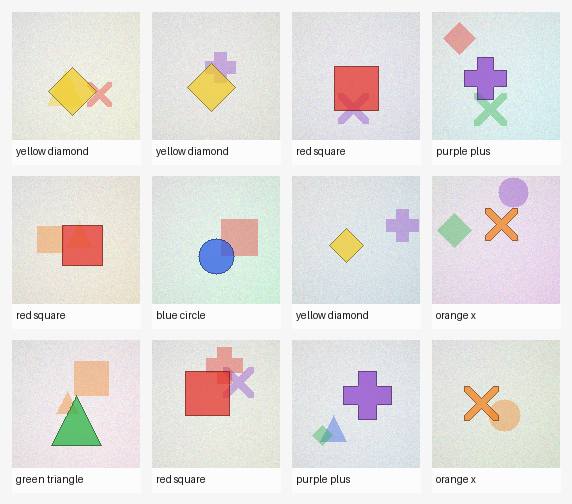
\includegraphics[width=0.82\linewidth]{figures/clip_train_examples.png}

\small Representative training examples for the CLIP problem, with class labels shown below each image.
\end{center}

\medskip
\noindent\textbf{Pretrained CLIP model.}
Use Hugging Face \texttt{AutoProcessor} and \texttt{CLIPModel} with one of the provided CLIP checkpoints.
The intended pattern matches the lecture notebook:
\begin{itemize}
\item load the processor and model from \texttt{from\_pretrained(...)},
\item build text embeddings for prompted class names,
\item encode images and compare image-text similarity scores,
\item use frozen image features for a linear probe.
\end{itemize}
Use the standard prompt template ``a photo of a class name'' as part of your prompted zero-shot setup.
The autograder is expected to have the selected CLIP checkpoint available through the Hugging Face cache for any feature generation done by the course staff.

\medskip
\noindent\textbf{Few-shot protocol.}
After loading pretrained CLIP, you will:
\begin{itemize}
\item evaluate zero-shot classification using prompted class names,
\item freeze the image encoder,
\item train a linear probe on the few-shot training split using configuration A,
\item retrain on \texttt{train+val} with the same configuration and save one checkpoint containing only the linear probe weights and minimal metadata.
\end{itemize}

\medskip
\noindent\textbf{Autograder.}
Gradescope will:
\begin{itemize}
\item run unit tests on the four core functions above,
\item run your training script,
\item load \texttt{outputs/clip\_model.pt},
\item use course-provided hidden CLIP features for the test split when available,
\item evaluate the submitted checkpoint on the hidden test split.
\end{itemize}
The score breakdown is:
\begin{itemize}
\item 40 points for correct implementations of the four core functions,
\item 10 points for reporting the requested validation numbers from \texttt{--mode train} in the required format.
\end{itemize}

\begin{enumerate}

\item \textbf{\texttt{build\_model\_and\_processor}: pretrained CLIP loading (10 points).}\\
Implement \texttt{build\_model\_and\_processor(model\_name, device)}.
It should load a pretrained \texttt{AutoProcessor} and \texttt{CLIPModel}, move the model to the requested device, and set evaluation mode.

\item \textbf{\texttt{build\_text\_features}: prompted class prototypes (10 points).} \\
Implement \texttt{build\_text\_features(...)}.
For each class name, encode all prompt templates, normalize template features, average them, and renormalize the final class prototype.

\item \textbf{\texttt{extract\_image\_features}: frozen CLIP feature extraction (10 points).}\\
Implement \texttt{extract\_image\_features(...)}.
It should iterate over a dataset, preprocess images with the CLIP processor, compute normalized frozen image features, and return the full feature matrix and label vector.

\item \textbf{\texttt{train\_linear\_probe}: few-shot classifier training (10 points).}\\
Implement \texttt{train\_linear\_probe(...)}.
Train a linear classifier on frozen CLIP image features with AdamW, evaluate on the validation split after each epoch, and keep the best probe by validation loss (tie-break by validation accuracy).

\item \textbf{Training-Mode Report and Checkpoint Submission (10 points).}\\
Run the provided script in \texttt{--mode train} and report the validation numbers it prints.
Your submitted report should include:
\begin{itemize}
\item the zero-shot validation loss and accuracy,
\item the validation loss and accuracy for all few-shot settings,
\item the final \texttt{fewshot-10} validation result.
\end{itemize}
Students do not have access to the hidden test split. Submit \texttt{outputs/clip\_model.pt} to Gradescope, and the autograder will evaluate it on hidden test data, which will be part of the grading.

\begin{solution}

\begin{tabular}{lccc}
\hline
Method & Config & Val loss & Val acc \\
\hline
Zero-shot CLIP & -- & 1.2392 & 0.6167 \\
Linear probe & fewshot-1 & 0.6162 & 0.8333 \\
Linear probe & fewshot-2 & 0.4324 & 0.9167 \\
Linear probe & fewshot-4 & 0.3911 & 0.9333 \\
Linear probe & fewshot-8 & 0.2886 & 0.9667 \\
Linear probe & final-fewshot-10 & 0.0865 & 1.0000 \\
\hline
\end{tabular}


\bigskip

For the test mode, we want to give grade based on percentage of average accuracy over base average accuracy 0.85 which is below, truncate at 1.

test-zeroshot: loss=1.3258 acc=0.5133
test-fewshot-1shot: loss=0.7864 acc=0.7733
test-fewshot-2shot: loss=0.6801 acc=0.7733
test-fewshot-4shot: loss=0.5333 acc=0.8633
test-fewshot-8shot: loss=0.4430 acc=0.8967
test-fewshot-10shot: loss=0.3091 acc=0.9567
test-fewshot-avg: loss=0.5504 acc=0.8527



\end{solution}

\end{enumerate}
\end{Q}
